\documentclass{article}

% --- load packages ---
\usepackage[margin=1in]{geometry} % change the margins
\usepackage{amsmath} % useful math environments and commands like align
\usepackage[colorlinks,bookmarks,bookmarksnumbered,allcolors=blue]{hyperref} % hyperlinks between references
\usepackage{graphicx}  % include images
\usepackage[table,xcdraw]{xcolor}
\usepackage[caption=false]{subfig} % subfigures.  false option prevents conflicts in caption styling with other packages
\usepackage{booktabs} % better tables
\usepackage[capitalise]{cleveref} % better referencing. uses cref.
\usepackage[section]{placeins} % sometimes useful to prevent figures from floating out of a section
\usepackage{cite} % handles multiple citations in one command better
\usepackage{doi} % allow correct hypderlinking of DOIs
\usepackage[normalem]{ulem}
\usepackage{float}

%\usepackage{minted} % for code highlighting
%\usepackage{lmodern}

\useunder{\uline}{\ul}{}


\begin{document}

\title{Optimal Spring Sizing}
\author{Landon Wright}
% put in \date{} if you don't want a date to appear, or enter a specific date, otherwise default is today's date.
\maketitle
\begin{centering}
\section*{Summary}

\end{centering}
\subsection{Design variable values}
The optimal cost was found to be \$400,140.
The determined optimum values for the design variables are as follows:

\begin{table}[H]
\centering
\caption{Optimum values for design}
\label{tab:optimum values}
\begin{tabular}{ll}
\hline
\textbf{Variable}      & \textbf{Value} \\
\hline
Velocity & $7.8161 \frac{ft}{s}$ \\
Pipe Diameter & $0.1816 ft$ \\
Particle Size  & $0.0005 ft$    \\
Water Flow Rate   & $0.1128 \frac{ft^{3}}{s}$\\
Volumetric Concentration & $0.4$\\
Slurry Density & $104.84 \frac{lbm}{ft^{3}}$\\

\hline
\end{tabular}
\end{table}

\subsection{Design function values}
\begin{table}[H]
\centering
\caption{Values of design functions at optimum}
\label{my-label}
\begin{tabular}{ll}
\hline
\textbf{Design Function}                       & \textbf{Value} \\
\hline\\
Maximize $F_{0}$                               & $6.4541 lbs$                    \\
$h_{S} + 0.05 \leq h_{def}$                    & $0.60 in \leq 0.60 in$          \\
$\tau_{a} \leq \frac{s_{e}}{s_{f}}$            & $18352 psi \leq 30000 psi$      \\
$\tau_{a} + \tau_{m} \leq \frac{s_{y}}{s_{f}}$ & $70576 psi \leq 70576psi$       \\
$4 \geq \frac{D}{d} \leq 16$                   & $4 in \leq 9.359 in \leq 16 in$ \\
$D + d \leq 0.75$                              & $0.75 in \leq 0.75in$           \\
$\tau_{solid} \leq s_{y}$                      & $75165 psi \leq 105860 psi$     \\
\hline  
\end{tabular}
\end{table}
\subsection{Binding Constraints}
The binding constraints are:
\begin{itemize}
    \item $h_{S} + 0.05 \leq h_{def}$
    \item $D + d \leq 0.75$
    \item $\tau_{a} + \tau_{m} \leq \frac{s_{y}}{s_{f}}$
\end{itemize}


\newpage
\section{Setup}
\subsection{Variable Mapping}
\begin{table}[H]
\centering
\caption{My caption}
\label{my-label}
\begin{tabular}{l@{\hskip 2in}l}
\underline{\textbf{Analysis Variables}} & \underline{\textbf{Design Variables}}                             \\
Wire Diameter               & Wire Diameter                                           \\
Coil Diameter               & Coil Diameter                                           \\
Number of Coils             & Number of Coils                                         \\
Free height                 & Free height                                             \\
Preload Height              &                                                         \\
Preload Deflection          &                                                         \\
Shear Modulus               &                                                         \\
Safety Factor               &                                                         \\
Endurance Limit             &                                                         \\
                            &                                                         \\
\underline{\textbf{Analysis Functions}} & \underline{\textbf{Design Functions}}       \\
Force                       & Maximize                                                \\
Spring Stiffness            & Solid Height $\leq$ Deflected height                    \\
Whal Factor                 & Alternating Stress $\leq \frac{s_{e}}{s_{f}}$           \\
Solid Height                & Alternating and Mean Stress $\leq \frac{s_{y}}{s_{f}}$  \\
Alternating Stress          & 4 $\leq$ Coil to Wire Ratio $\leq$ 16                   \\
Mean Stress                 & Solid Stress $\leq s_{y}$                               \\
Yield Strength              &                                                         \\
Coil to Wire Ratio          &                                                         \\
Spring Diameter             &                                                         \\
Deflected Height            &                                                        
\end{tabular}
\end{table}


\section{Results}
\subsection{Optimum values of variables and functions}
\begin{table}[H]
    \centering
    \caption{Optimum Values of Variables and Functions (binding functions are highlighted)}
    \label{tab:optimums}
    \begin{tabular}{ll}
    \hline
        \textbf{Variable/Function} & \textbf{Value}\\
    \hline
        Wire Diameter & 0.0724 in \\
        Coil Diameter & 0.6776 in \\
        Number Coils  & 0.5928    \\
        Free Height   & 1.3691   \\
        Preload Height & 1.0 in\\
        $\delta_{0}$ & 0.4 in\\
        $h_{def}$ & 0.6 in\\
        \cellcolor[HTML]{FFFE65}{\color[HTML]{333333}$h_{s}$} & 0.55in\\
        $F_{0}$ & 6.454 lbs\\
        k & 17.4853 lbs/in\\
        K & 1.1561\\
        $\tau_{max}$ & 70576 psi\\
        $\tau_{min}$ & 33871 psi\\
        $\tau_{a}$ & 18353 psi\\
        $\tau_{m}$ & 52224 psi\\
        \cellcolor[HTML]{FFFE65}{\color[HTML]{333333}$\tau_{a} + \tau_{m}$} & 70576 psi\\
        $\frac{S_{e}}{S_{f}}$ & 30000 psi\\
        $\frac{S_{y}}{S_{f}}$ & 70576 psi\\
        $\frac{D}{d}$ & 9.3539\\
        \cellcolor[HTML]{FFFE65}{\color[HTML]{333333}$D + d$} & 0.75\\
    \hline
    \end{tabular}
\end{table}


\subsection{Starting points and obtained values}

\begin{table}[H]
\centering
\caption{Optimized Values from Given Starting Point}
\label{tab:tries}
\resizebox{\textwidth}{!}{%
\begin{tabular}{l|llll|llll}
      & \multicolumn{4}{c}{{\textbf{Initial Values}}}             & \multicolumn{4}{c}{{\textbf{Optimized Values}}}           \\
      \hline
Trial & Wire Diameter & Coil Diameter & Number of Coils & Free Height & Wire Diameter & Coil Diameter & Number of Coils & Free Height \\
\hline
1     & 0.04735309758 & 0.2632045077  & 13.47275949     & 1.525959964 & 0.07243674785 & 0.6775631377  & 7.592829475     & 1.369115417 \\
2     & 0.07681530634 & 0.6400386081  & 12.94948955     & 1.594751247 & 0.07243674785 & 0.6775631377  & 7.592829475     & 1.369115417 \\
3     & 0.1842667961  & 0.2857953622  & 15.87240389     & 1.778356185 & 0.07243674785 & 0.6775631377  & 7.592829475     & 1.369115417 \\
4     & 0.08228471093 & 0.4690840665  & 4.289522923     & 1.148555107 & 0.07243674785 & 0.6775631377  & 7.592829475     & 1.369115417 \\
5     & 0.1108515351  & 0.6064586996  & 18.87818163     & 1.216915588 & 0.07243674785 & 0.6775631377  & 7.592829475     & 1.369115417 \\
6     & 0.1180764956  & 0.4051039167  & 3.202335182     & 1.40341038  & 0.07243674785 & 0.6775631377  & 7.592829475     & 1.369115417 \\
7     & 0.04081463856 & 0.6162849514  & 8.290655715     & 1.575679822 & 0.07243674785 & 0.6775631377  & 7.592829475     & 1.369115417 \\
8     & 0.0414732586  & 0.4912882619  & 7.470511837     & 1.688671189 & 0.07243674785 & 0.6775631377  & 7.592829475     & 1.369115417 \\
9     & 0.1409507556  & 0.5862985353  & 10.65920717     & 1.17543924  & 0.07243674785 & 0.6775631377  & 7.592829475     & 1.369115417 \\
10    & 0.05350562406 & 0.693669285   & 5.590426322     & 1.84323528  & 0.07243674785 & 0.6775631377  & 7.592829475     & 1.369115417 \\
\hline
\end{tabular}%
}
\end{table}


\subsection{Design space contour plot}
\begin{figure}[H]
    \centering
    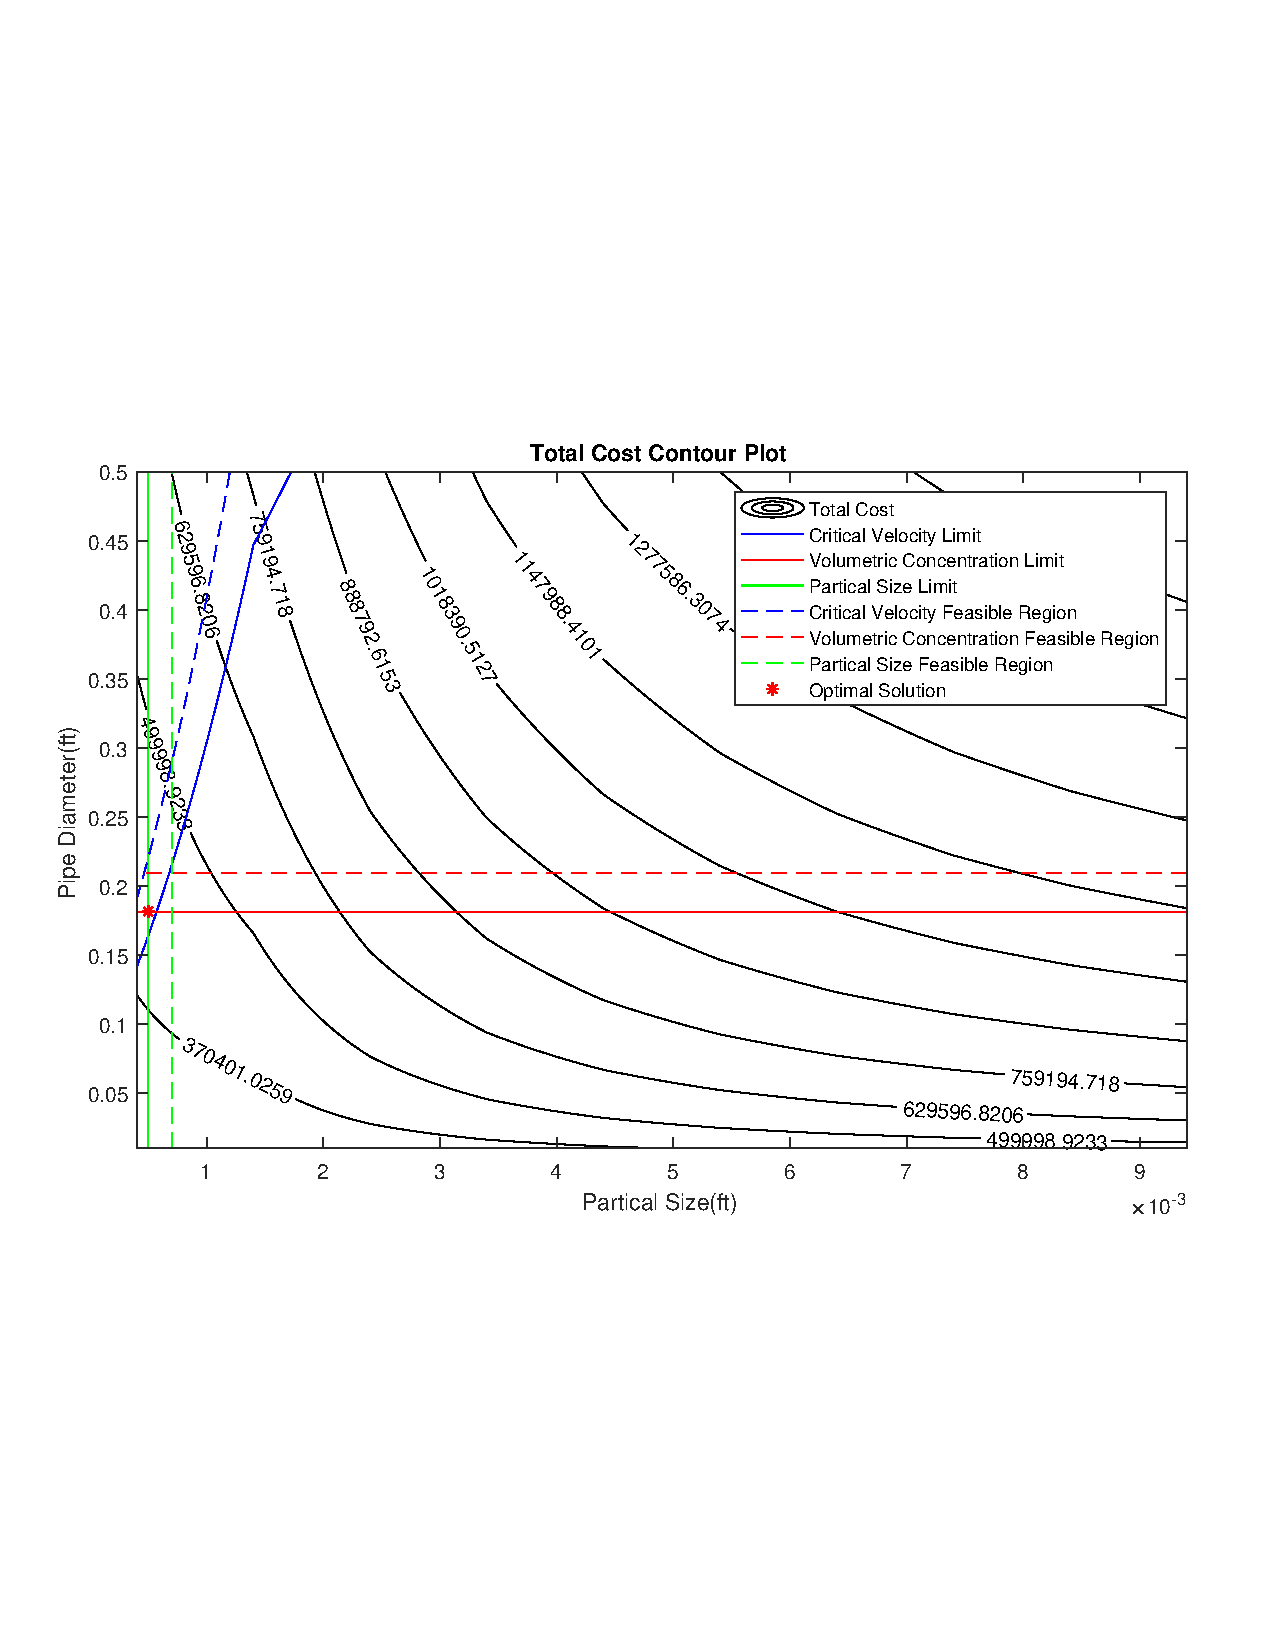
\includegraphics[width=3.in]{PlotBig.pdf}
    \caption{Contour plot showing the design space}
    \label{fig:big}
\end{figure}

\subsection{Feasible design space contour plot}
\begin{figure}[H]
    \centering
    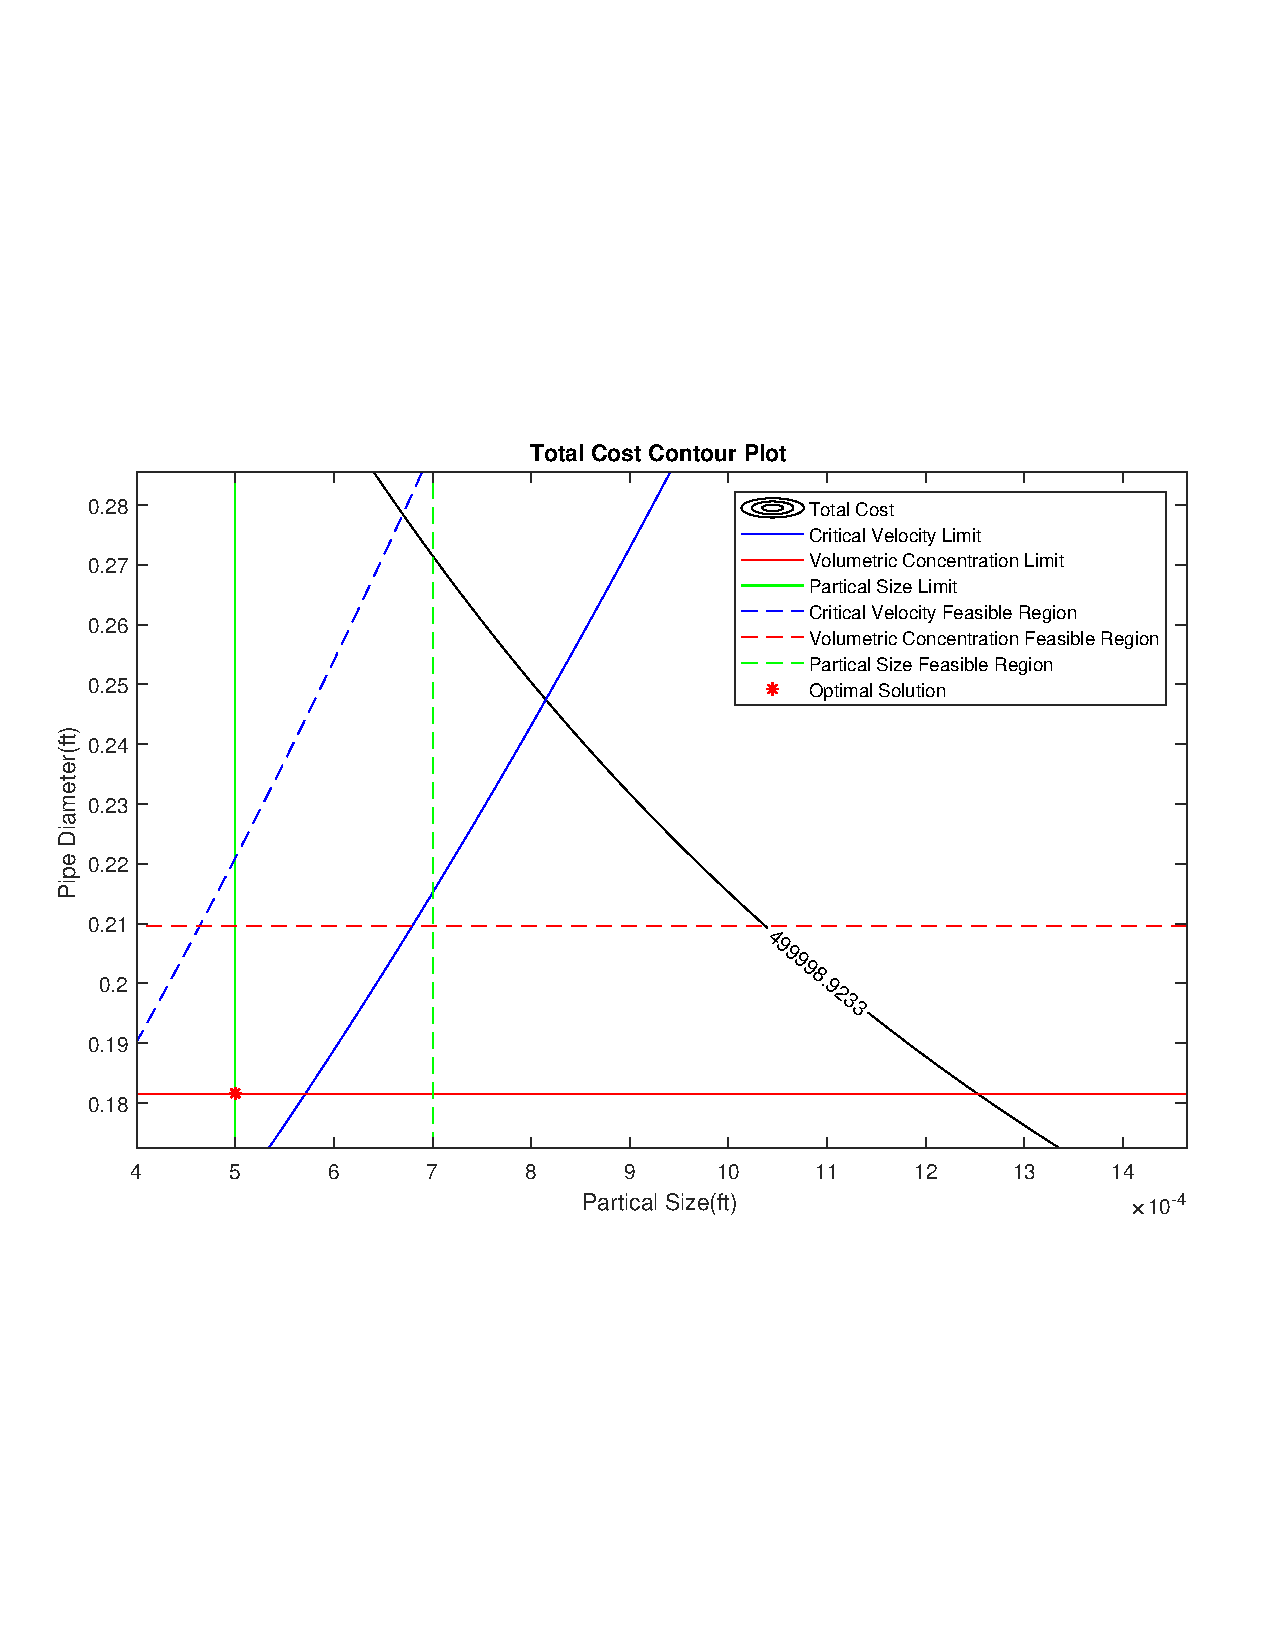
\includegraphics[width=3.in]{PlotZoomed.pdf}
    \caption{Contour plot showing the feasible design space}
    \label{fig:close}
\end{figure}

\section{Discussion}
As can be seen in figure \ref{fig:big} the design space for this problem is quite restricted.  There are several contraints and the feasible design space is quite small compared to the total design space, at least when viewed on a contour plot of wire diameter and spring diameter.  Due to the fact that the contours shown in Figure \ref{fig:big} are quite linear and that the various initial values tried all converged to the same value as shown in Table \ref{tab:tries} I conclude that we have found a global optimum for the spring given the applied constraints.  It is also of interest that the optimum appears to be bound by three constraints, meaning that if we wanted to increase the increase the rate of the spring by only changing the spring or wire diameter we would need to either relax the alternating and mean stress constraint(ie. find a stronger material), or we would need to relax both the solid height and spring size constraints.  It is important to remember that Figures \ref{fig:big} and \ref{fig:close} are only showing a portion of the design space and other options should also be considered


\section{Appendix}

\subsection{Matlab files}
\subsubsection{Optmization code}
\subsubsection{Plotting Code}
\end{document}
\textbf{}